%%%%%%%%%%%%%%%%%%%%%%%%%%%%%%%%%%%%%%%%%%%%%%%%%%%%%%%%%%%%%%%
\chapter{Crystal Structure in Solids}

Solids tend to arrange themselves into ordered, repeating structures. These can be conveniently described mathematically in the ways laid out in this chapter.



\begin{definition}
{lattice}{set of mathematical points to which the basis is attached}
\end{definition}

A lattice is defined by three translation vectors $\mathbf{a}_1, \mathbf{a}_2, \mathbf{a}_3$, such that integer $u_1, u_2, u_3$ movement along these are equivalent points:
\begin{equation} \label{eq:lattice-translation}
    \mathbf{r}' = \mathbf{r} + u_1\mathbf{a}_1 + u_2\mathbf{a}_2 + u_3\mathbf{a}_3
\end{equation}

\begin{definition}
{basis}{identical group (of atoms) that repeated infinitely to fill space}
\end{definition}
The position of the atom (or atoms) in the basis can be described by the position vector:
\begin{equation}
    \mathbf{r}_j = x_j\mathbf{a}_1 + y_j\mathbf{a}_2 + z_j\mathbf{a}_3 \;: \; 0 \leq x_j, y_j, z_j \leq 1 
\end{equation}

\begin{definition}
{primitive lattice}{Any two points from which the atomic arrangement looks the same satisfy \ref{eq:lattice-translation} with a suitable choice of the integers $u_i$}
\end{definition}
\begin{definition}
{primitive translation vectors}{Translation vectors $\mathbf{a}_i$ that satisfy the definition of the primitive lattice.}
\end{definition}

\begin{definition}
{crystal axes}{The set of primitive translation vectors that form the three adjacent edges of the primitive parallelepiped}
\end{definition}
It is often most convenient to use the crystal axes as the coordinate system in crystalline solids. The primitive translation vectors define the \emph{smallest volume} cell that can fill space with primitive translations. This volume is
\begin{equation}
    V_c = |\mathbf{a}_1 \cdot \mathbf{a}_2 \times \mathbf{a}_3|
\end{equation}

\begin{definition}
{primitive cell}{smallest-volume cell that will fill all space by primitive lattice translations. No basis contains fewer atoms than the primitive basis, and a primitive cell contains one lattice point.}
\end{definition}

\begin{definition}
{Wigner-Seitz Cell}
{primitive cell that can be constructed by the method:
\begin{enumerate}
    \item Draw vectors from a lattice point to its neighbors.
    \item Draw planes bisecting the vectors from step 1.
    \item Take the smallest volume enclosed by these planes.
\end{enumerate}
}
\end{definition}

\begin{figure}[h]
    \centering
    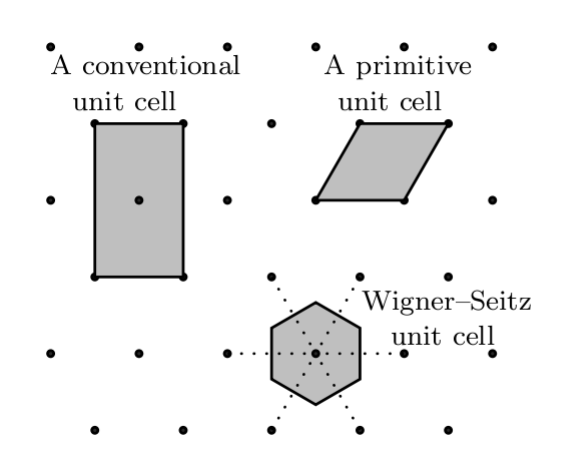
\includegraphics[width=0.5\textwidth]{./figures/wigner-seitz-ex.png}
    \caption{An example from lecture slides for Wigner-Seitz cell.}
    \label{fig:wigner-seitz-ex}
\end{figure}



%--------------------------------------------%
\section{Lattice Types}
A crystal lattice is repeated by translation vectors $\mathbf{T}$ and by various other symmetry operations. 
\begin{definition}
{Mirror Symmetry}{$(m)$ Reflection in a plane}
\end{definition}
\begin{definition}
{Inversion Symmetry}{$(\Bar{1})$ Reflection in a point}
\end{definition}
\begin{definition}
{N-fold Rotational Symmetries}{$(C_n)$ Rotations of $2\pi/n$ about point}
\end{definition}

\begin{theorem}
The only allowed rotational symmetries in a discrete lattice are 2-fold, 3-fold, 4-fold, and 6-fold.
\end{theorem}
Although molecules can have any rotational symmetries, there is a theorem about the allowed rotational symmetries in a lattice. We had to prove this for a two-dimensional lattice on our homework, but a helpful webpage \href{http://www.xtal.iqfr.csic.es/Cristalografia/parte_03_1_1-en.html}{here} explains it well.

\begin{definition}
{Bravais Lattice}{common phrase for distinct lattice types. There are 5 in two dimensions and 14 in three dimensions.}
\end{definition}

%--------------------------------------------%
\subsubsection{Two-Dimensional Lattice Types}
\begin{table}[h]
    \centering
    \begin{tabular}{l|c|c}
        \textbf{Name} & \textbf{Distances} & \textbf{Angles} \\
        \hline
        Oblique      & $|a_1|\neq |a_2|$ & \\
        Square       & $|a_1|=|a_2|$     & $\phi=\pi/2$ \\
        Rectangular  & $|a_1|\neq |a_2|$ & $\phi=\pi/2$ \\
        Hexagonal    & $|a_1|=|a_2|$     & $\phi=2\pi/3$ \\
        Centered Rectangular  & $|a_1|\neq |a_2|$ & $\phi=\pi/2$
    \end{tabular}
    \caption{Bravais Lattice types in two dimensions.}
    \label{tab:2d-bravais}
\end{table}
A centered rectangular lattice is a rectangular lattice with a lattice point in the center of it.

%--------------------------------------------%
\subsubsection{Three-Dimensional Lattice Types}
\begin{table}[h]
    \centering
    \begin{tabular}{l|c|c|c}
        \textbf{Name} & \textbf{Lattices} & \textbf{Distances} & \textbf{Angles} \\
        \hline
        Triclinic    & 1 & $|a_1|\neq |a_2|\neq |a_3|$ & $\alpha\neq\beta\neq\gamma$ \\
        Monoclinic   & 2 & $|a_1|\neq |a_2|\neq |a_3|$ & $\alpha=\gamma=\pi/2\neq\beta$ \\
        Orthorhombic & 4 & $|a_1|\neq |a_2|\neq |a_3|$ & $\alpha=\beta=\gamma=\pi/2$ \\
        Tetragonal   & 2 & $|a_1|=|a_2|\neq |a_3|$     & $\alpha=\beta=\gamma=\pi/2$ \\
        Cubic        & 3 & $|a_1|=|a_2|=|a_3|$         & $\alpha=\beta=\gamma=\pi/2$ \\
        Trigonal     & 1 & $|a_1|=|a_2|=|a_3|$         & $\alpha=\beta=\gamma<2\pi/3,\neq\pi/2$ \\
        Hexagonal    & 1 & $|a_1|=|a_2|\neq |a_3|$     & $\alpha=\beta=\pi/2,\; \gamma=2\pi/3$ \\
    \end{tabular}
    \caption{Bravais Lattice types in three dimensions.}
    \label{tab:3d-bravais}
\end{table}


%--------------------------------------------%
\subsection{Cubic Lattices}
The three cubic lattices are simple cubic (sc), body-centered cubic (bcc), and face-centered cubic (fcc). Some useful properties are summarized in the table below.

\begin{table}[h!]
    \centering
    \begin{tabular}{l|c|c|c}
        \textbf{Property} & \textbf{Simple} & \textbf{Body-centered} & \textbf{Face-centered} \\
        \hline
        Lattice points per cell & 1 & 2 & 4 \\
        Volume of primitive cell & $a^3$ & $a^3/2$ & $a^3/4$ \\
        Number of nearest neighbors & 6 & 8 & 12 \\
        Packing fraction &  $\frac{1}{6}\pi$ & $\frac{\sqrt{3}}{8}\pi$ & $\frac{\sqrt{2}}{6}\pi$
    \end{tabular}
    \caption{Some properties of cubic lattices.}
    \label{tab:cubic-properties}
\end{table}

Cubic systems have the highest number of symmetries. They are:
\begin{enumerate}
    \item Inversion symmetry for center of cell $(C_i)$
    \item Six mirror planes $(C_s)$
    \item Three 4-fold symmetry axes $(C_4)$
    \item Four 3-fold axes $(C_3)$
    \item Four 2-fold axes $(C_2)$
\end{enumerate}
%--------------------------------------------%
\subsubsection{Primitive Cubic Lattice}
The primitive cell of the \emph{simple cubic} cell is itself, with lattice vectors:
\begin{equation*}
    \mathbf{a}_1 = a \hat{\mathbf{x}} \quad \mathbf{a}_2 = a \hat{\mathbf{y}} \quad \mathbf{a}_3 = a \hat{\mathbf{z}}
\end{equation*}

%--------------------------------------------%
\subsubsection{Body-Centered Cubic Lattice}
Examples include alkali metals, Ba, Nb, W, and bcc Cr or Fe. The Wigner-Seitz cell of the \emph{body-centered cubic} cell is a \emph{truncated octahedron}, with lattice vectors:
\begin{align*}
    \mathbf{a}_1 & = \frac{1}{2} a (\hat{\mathbf{x}} + \hat{\mathbf{y}} - \hat{\mathbf{z}}) \\
    \mathbf{a}_2 & = \frac{1}{2} a (-\hat{\mathbf{x}} + \hat{\mathbf{y}} + \hat{\mathbf{z}}) \\
    \mathbf{a}_3 & = \frac{1}{2} a (\hat{\mathbf{x}} - \hat{\mathbf{y}} + \hat{\mathbf{z}}) 
\end{align*}

%--------------------------------------------%
\subsubsection{Face-Centered Cubic Lattice}
Examples include Cu, Ag, Au, Ni, Pd, Pt, and Al. The Wigner-Seitz cell of the \emph{face-centered cubic} cell is a \emph{rhombic dodecahedron}, with lattice vectors:
\begin{align*}
    \mathbf{a}_1 & = \frac{1}{2} a (\hat{\mathbf{x}} + \hat{\mathbf{y}}) \\
    \mathbf{a}_2 & = \frac{1}{2} a (\hat{\mathbf{y}} + \hat{\mathbf{z}}) \\
    \mathbf{a}_3 & = \frac{1}{2} a (\hat{\mathbf{x}} + \hat{\mathbf{z}}) 
\end{align*}



%--------------------------------------------%
\section{Index System for Crystal Planes}
Crystal planes can be defined by their intercepts
\begin{equation*}
    S_1 = m_1 \mathbf{a} \quad S_2 = m_2 \mathbf{b} \quad S_3 = m_3 \mathbf{c}
\end{equation*}

\subsubsection{Miller index}
The common system for indexing planes in a lattice. They are found by the method below.
\begin{enumerate}
    \item Calculate the reciprocal values $\frac{1}{m_1}$, $\frac{1}{m_2}$, $\frac{1}{m_3}$
    \item Multiply those values with the smallest integer $p$, which turns the values into integers $h=\frac{p}{m_1}$, $k=\frac{p}{m_2}$, and $l=\frac{p}{m_3}$
    \item The index of the plane is $(hkl)$\footnote{Negative intercepts are denoted with a bar above the index.}
\end{enumerate}

The normal vector of a set of planes is
\begin{equation*}
    \mathbf{n} = h \, \mathbf{a} + k \, \mathbf{b} + l \, \mathbf{c} \equiv [hkl]
\end{equation*}



%--------------------------------------------%
\section{Atomic Packing Factor}
\begin{definition}
{Atomic Packing Factor (APF)}{Fraction of cell volume that is occupied by atoms}
\end{definition}
\begin{equation}
    APF = \frac{N_{atoms}V_{atoms}}{V_{cell}}
\end{equation}

If one tries to construct the structure that is \emph{close-packed}, there are two options with $APF=0.74$. Stacking layers in the sequence $ABAB...$ leads to \emph{hexagonal close-packed} structure, and stacking in the sequence $ABCABC...$ gives the fcc structure.

\vspace{10pt}
\textbf{Note:} This chapter also included $NaCl$, $CsCl$, and Diamond structures as examples of simple lattices.